\section{Reading Assignment}

\subsection{Nennen Sie 5 verschiedene Quellen für Entropie}

\large
Physikalische Phänomene
\normalsize

\begin{itemize}
    \item Radioaktiver Zerfall
    \item Transmission von Photonen
    \item Thermisches Rauschen (Johnson-Nyquist-Rauschen)
    \item Geräusche der Atmosphäre
    \item Jitter
\end{itemize}


\large
Mensch-Gerät Interaktion
\normalsize

\begin{itemize}
    \item Dauer von Tastendrücken und andere Zeitmessungen
    \item Tasten-und Mausbewegungen
    \item Bewegungs- und Beschleunigungssensoren
\end{itemize}

\subsection{Wie viele Samples aus einem Smartphone Accelerator benötigen wir um einen 128 bit key zu
erstellen?}



\glqq Since the recommended security level for almost 
random bits is $\epsilon = 2^{-80}$. According to the 
heuristic (1) we need roughly 128/0.125  = 1024
samples to extract a 128-bit key. However taking into 
account the true error in our Theorem 1 we see that we 
need at least n ≈ 2214 bits!\grqq  \\~\\

Laut dem Paper, welches sie auf Theoreme stützt, 
braucht man mindestens 1024 Samples. Hinzu kommt 
allerdings, dass empfohlen wird, ein \textit{n} 
mit mehr als 2214 Bitlänge zu wählen.


\subsection{Wie groß ist der Unterschied an tatsächlich extrahierbarer Entropie und Shannon Entropie?}

\begin{figure}[hbt!]
	\centering
		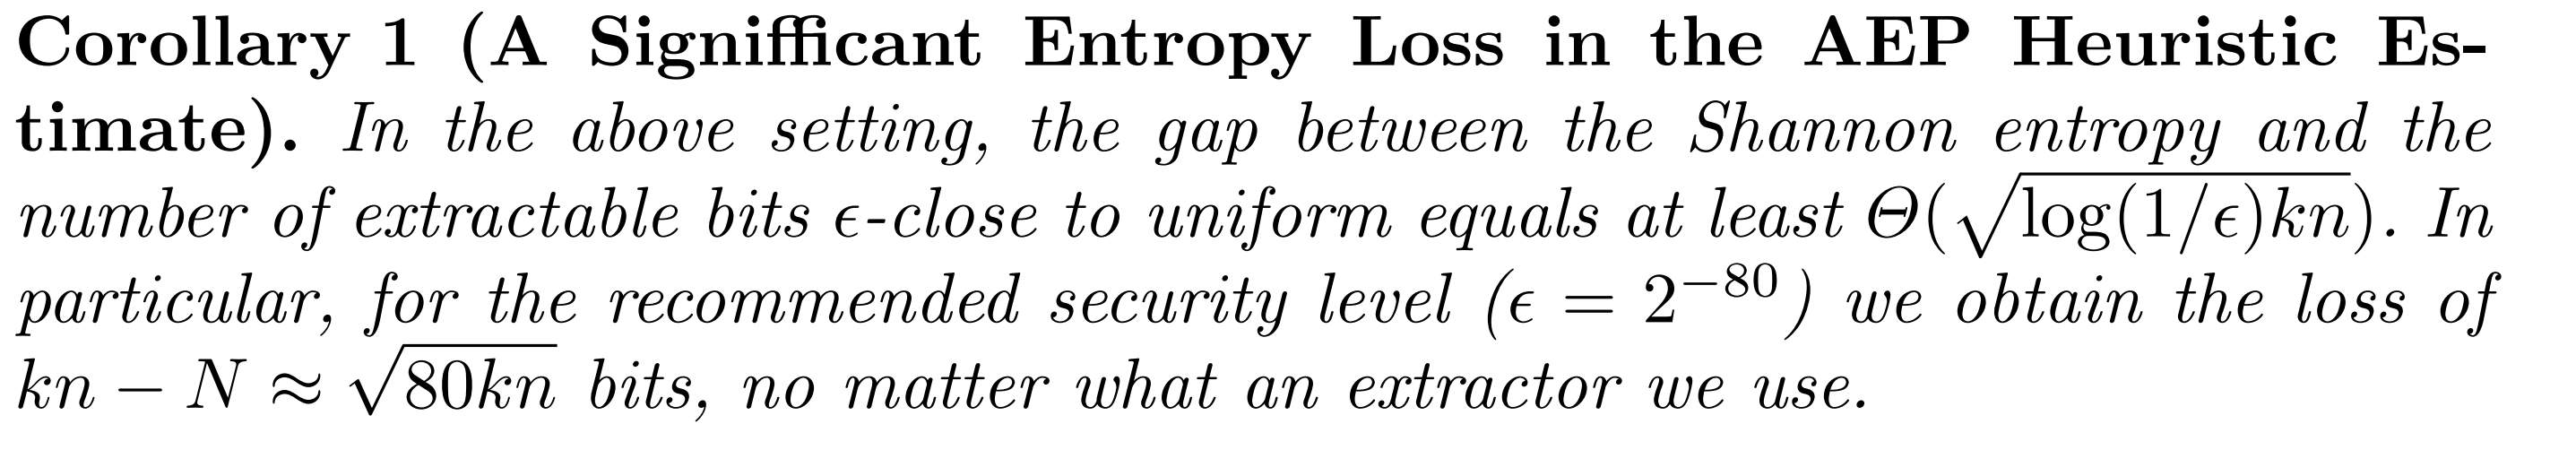
\includegraphics[width=1\textwidth ]
		{Bilder/a5-Corollary1.png}
		\caption{Auszug aus dem Paper}
		\label{fig:5.1}
\end{figure}
\clearpage

\glqq In information theory
most widely used is Shannon entropy, which quantifies 
the encoding length of a given distribution. In turn, 
cryptographers use the more conservative notion
called min-entropy, which quantifies unpredictability. 
In general, there is a large
gap between these two measures: the min-entropy of an 
n-bit string might be only
$O(1)$ whereas its Shannon entropy as big 
as $\Omega (n)$.\grqq \\    

Die min-Entropie eines n-bit langen stringes kann konstant
sein, wobei gleichzeitig seine Shannon Entropie linear oder
größer zu \textit{n} sein kann.\\\\

Von den 2214 bits können nur etwa 128 bits mit nahezu 
zufällig gleichverteilter Qualität extrahiert werden.
Das ist ein Verhältnis von $\frac{128}{2214} ≈ 0.0578$
oder anders gesagt: Der Schlüssel hat hier nur die Länge 
von 5,78\% von der Bitlänge des Samples.


